\documentclass[12pt]{article}

% Packages
\usepackage{packages}
\usepackage{commands}
\usepackage{titlepage}


% Title page parameters
\setToResearch
\setTitle{Прототип edtech-продукта «WORKSCHOICE»}
\setYear{2022}

% Document Beginning
\begin{document}

\makeTitlePage

{
  \hypersetup{linkcolor=black}
  \tableofcontents
}

\hypersetup{linkcolor=black}

\section{Идея проекта}

WorksChoice -- сервис по определению образовательной траектории студента, получению профессиональных знаний и помощи в освоении необходимого материала. 

WorksChoice -- платформа по дополнительному образованию с входным психологическим тестированием для студентов, курсами и с тьюторами, которые помогают студентам в процессе обучения и поддерживают их. Сервис помогает определиться с образовательной траекторией, а также предоставляет обучающие онлайн-курсы по большинству профессий с постоянной поддержкой со стороны тьюторов -- личных мотиваторов и помощников по учебе. 
Наша цель: помочь студенту определиться со своим профессиональным путем и обеспечить его необходимыми материалами для реализации его целей, а также повышать его личную мотивацию на протяжении всего обучения \cite{Kobzov}.

\subsection{Функционал платформы}
\begin{itemize}
    \item Входное психологическое тестирование: вступительный тест из 50 вопросов для определения сильных сторон и предрасположенностей ученика. По результатам теста формируются рекомендации для студентов по прохождению курсов, карта сильных и слабых сторон, а также подбираются профессии на основе интересов и личных особенностей студента. Для прохождения теста необходимо пройти предварительную регистрацию.
    \item Бесплатная база тестов и заданий по разным профессиям, чтобы пользователь мог оценить свой уровень в различных сферах. Более подробное тестирование ученик проходит по результатам прохождения курса.
    \item Личный кабинет: отображается количество пройденных курсов, показывается прогресс по каждому курсу (уровень прохождения курса рассчитывается на основе проверочных заданий после видеолекций).
    \item Тьюторы: профессионалы из разных сфер, которые готовы быть наставниками и трекерами для обучающихся. Они осуществляют мотивационную поддержку и проводят консультации с клиентом, если он не понимает некоторые аспекты выбранного курса. Тьюторы не являются преподавателями курсов. Тьютор помогает достигать планируемых целей. У одного тьютора может быть несколько студентов. Общение со студентами проводится в телеграмм-чатах, где находится непосредственно сам студент, его наставник и диспетчер сервиса, который следит за характером их общения, к которому также можно обратиться по техническим вопросам. 
    \item Каталог курсов. Основными компонентами каждого курса являются видеолекция и проверочные задания, однако в зависимости от профессии в курсе могут содержаться и дополнительные механики. По итогу прохождения профессионального курса платформа предоставляет диплом об освоенной профессии.
    \item Мастермайнд-группы: группа из 5 человек, которая собирается вместе в конце каждого месяца для обсуждения результатов участников группы. Студенты помогают другу другу в обмене идеями и развитии в процессе обучения, решают кейсы, выполняют групповые задания. Для работы используется доска Miro~\cite{Miro} и другие инструменты. Используются не для всех профессий. У каждой группы есть свой чат в телеграмме. 
\end{itemize}

\subsection{Обоснование актуальности продукта}

В 2019–2022 годах больше половины россиян в возрасте 17-22 года, проживающих в крупных городах, проходили какое-либо дополнительное онлайн-обучение. Из тех, кто получает дополнительное онлайн-образование, в основном студенты хотят повысить квалификацию, получить дополнительную профессию, или открыть свой бизнес. Многие выпускники школ не могут чётко сформулировать свои карьерные предпочтения, а некоторые идут в университет под давлением внешних обстоятельств. Таким образом, спрос на онлайн-курсы с каждым годом растёт, и в связи с пандемией этот тренд только усилился. По оценкам авторов исследования EdMarket Research, российский рынок онлайн-образования последние пять лет растет примерно на 20\%: в 2016 году он оценивался в 20,7 млрд рублей, а к 2021 году достигнет 53,3 млрд~\cite{RussianEdtechStudy2022}. 

По данным исследования российского рынка онлайн-образования, которое провел проект «Барометр», чаще всего дистанционные курсы длятся от одного до трех месяцев. Ситуация, когда студент бросает проходить купленный онлайн курс, — частое явление: до конца курса в среднем доходят всего 59\% студентов~\cite{VentureInvesting}.

Таким образом, спрос на услуги онлайн-образования крайне высок, однако, к сожалению, в сфере Edtech очень много людей студенческого возраста не проходят курсы до конца, бросают: покупают, а потом забывают, что им курс был актуален. Наш сервис пытается решить эту проблему с помощью тьюторов, которые сопровождают учеников на протяжении всей работы с нашей платформой. Социальная значимость нашей платформы заключается в решении проблемы неэффективной занятости. Научные исследования показывают, что взвешенная оценка подлинного характера профориентации студента является важным условием для повышения эффективной занятости в стране~\cite{VentureInvesting},~\cite{Donetsky}.

\subsection{Анализ целевой аудитории}

\begin{itemize}
    \item Студенты. Портрет ЦА: люди от 17 до 22 (24) лет; могут подрабатывать, либо находиться на попечении у родителей; скорее всего имеют опыт онлайн-образования, так как готовились к ЕГЭ; плохо ориентируются в edtech-продуктах; стремятся получить профессию и быть востребованными на рынке; идеальный результат для них -- получение знаний и навыков, которые можно применять на практике~\cite{TinkoffStudy};
    \item Люди с высшим образованием, которым не нравится их специальность, либо они хотят получить дополнительные навыки для своей профессии. Портрет ЦА: люди в возрасте от 24 до 40 лет; живут в городе-миллионнике; работают в офисе; уровень дохода средний: 30–70 тысяч рублей; могут не иметь опыта в онлайн-образовании и плохо ориентируются в edtech-продуктах~\cite{TinkoffStudy};
    \item Люди, которые учится не ради карьеры, а просто для удовольствия или расширения кругозора. Портрет ЦА: люди от 25 до 35 лет, есть стабильный заработок, имеют обширный опыт в онлайн-образовании; могут ориентироваться в edtech-продуктах~\cite{TinkoffStudy};
\end{itemize}

Наш сервис ориентирован прежде всего на студентов. Однако, безусловно, мы учитываем и другие категории клиентов, которые потенциально может охватить наша платформа. Устройство нашего продукта позволяет работать и с другими категориями ЦА, так как при необходимости пользователь может отказаться от прохождения входного психологического тестирования и от тьютора, если считает, что ему это не нужно, и сразу перейти к курсам. 

\section{Обзор рынка}

\subsection{Проблемы, которые решает наш продукт}
\begin{itemize}
    \item Проблема профессионального самоопределения и точного выбора образовательного пути. Сервис помогает определиться с образовательной траекторией без перебора сотни курсов и без разочарования в образовании, ускоряет выявление способностей и перспектив саморазвития.
    \item Проблема демотивации. Также платформа решает проблему мотивации благодаря тьюторам, которые поддерживают и помогают ученику во время всего обучения по специальности. Входное профориентационное тестирование позволяет определить настоящие предпочтения и сильные стороны человека и на основе этих данных предложить ему профессии, которые ему будет комфортно постигать, что также способствует росту личной мотивации.
    \item Проблема неэффективной занятости. Данная ситуация является производной из двух вышеперечисленных. Эту проблему наша платформа решает не только уже упомянутыми способами, но и наличием каталога курсов по разным профессиям. Даже если специалист чувствует себя на своём месте и у него нет проблем с мотивацией, он может про себя понимать, что его образования может быть недостаточно в некоторых аспектах. Благодаря нашим курсам человек сможет повысить свою квалификацию, повысив эффективность в текущей сфере занятости.
\end{itemize}


\subsection{Основные конкуренты}

\begin{longtable}{|p{3.5cm}|p{3.5cm}|p{4.3cm}|p{4.3cm}|}
\hline
\textbf{Название} & \textbf{Продукт} & \textbf{Преимущества} & \textbf{Недостатки} \\
\hline
\endfirsthead
\multicolumn{4}{c}
{\tablename\ \thetable\ -- \textit{Продолжена с предыдущей страницы}} \\
\hline
\textbf{Название} & \textbf{Продукт} & \textbf{Преимущества} & \textbf{Недостатки} \\
\hline
\endhead
\hline \multicolumn{4}{r}{\textit{Продолжена на следующей странице}} \\
\endfoot
\hline
\endlastfoot
\begin{nohyphens}
Skillbox~\cite{Skillbox}
\end{nohyphens}
&
\begin{nohyphens}
\RaggedRight 1. Каталог курсов по разным профессиям; \newline
2. Тест на профориентацию; \newline
3. Школа кураторов;
\end{nohyphens}
&
\begin{nohyphens}
{\RaggedRight 1. Курсы с трудоустройством; \newline
2. Стажировки в компаниях; \newline
3. Практика; \newline
4. Вебинары;
}
\end{nohyphens}
& 
\begin{nohyphens}
{\RaggedRight 1. Некачественный контент; \newline
2. Много негативных отзывов о курсах; \newline
3. Нет помощи в построении образовательной траектории; \newline
4. Нет теста на определение сильных сторон; \newline
5. Нет наставника, который сопровождает студента во время обучения;
}
\end{nohyphens}
 \\
 \begin{nohyphens}
 Нетология~\cite{Netology}
 \end{nohyphens}&
 \begin{nohyphens}
{\RaggedRight 1. Курсы по навыкам и профессиям;\newline
2. Диплом о высшем образовании;\newline
3. Переобучение в ИТ специалиста;
}
\end{nohyphens}
 & 
 \begin{nohyphens}
{\RaggedRight 1.Позиционирование, как интернет-университет; \newline
2. Трудоустройство в компании-партнеры;\newline
3. Переобучение на актуальные специальности;

}
\end{nohyphens}
 & 
  \begin{nohyphens}
{\RaggedRight 1. Нет возможности системно построить собственную образовательную траекторию;\newline
2. Нет входного психологического тестирования;\newline
3. Нет выделения конкретных целевых аудиторий курсов;\newline
4. Нет кураторов;

}
\end{nohyphens} \\
  \begin{nohyphens}
  Скиллфолио~\cite{Skillfolio}
  \end{nohyphens}&
{
\par
\RaggedRight1.Персонализиро\-ванное обучение и комплексная диагностика;\newline
2. Профориентация для подростков;\newline
3. Тьюторское сопровождение;\newline
4. Эксперт по развитию карьеры;
\par
}
 & 
  \begin{nohyphens}
{\RaggedRight1. Фокусная работа как сервиса по развитию софт скиллс;\newline
2. Много тестов по диагностике сильных сторон и направлений развития;\newline
3. Профориентация и курсы для компаний;

}
\end{nohyphens}
 & 
  \begin{nohyphens}
{\RaggedRight1. Небольшое количество курсов и программ;\newline
2. Фокус в основном только на развитии мягких навыков;\newline
3. Нет широкой линейки курсов;
}
\end{nohyphens} \\
\end{longtable}

\subsection{Преимущества нашего сервиса Workschoice:}
\begin{itemize}
    \item Психологическое тестирование: входное тестирование на сильные стороны и профессиональные сферы, к которым студент имеет предрасположенность.
    \item Персональный тьютор: трекер и личный учебный наствник, который помогает достигать образовательных результатов и профессиональных целей.
    \item Рекомендации по результатам анализа характера обучения студента на выбранной образовательной траектории: проводим анализ результатов студента в процессе обучения, помогаем выбрать правильные направления обучения после тестирования и общения с тьютором, отслеживаем результаты и успехи ученика онлайн, тьютор дает обратную связь по обучению, рекомендации о том, что получается лучше всего.
\end{itemize}

\section{Методология образовательного продукта}
Наш сервис помогает студентам определиться с их профессиональным путём с помощью входного психологического тестирования, которое ориентировано на максимально точное определение предрасположенности студента и предложение курсов, соответствующих его интересам. Далее будут рассмотрены образовательные формы и форматы, через которые ученик постигает профессию. Наша платформа будет содержать большой перечень курсов и, так как всех их отразить в коммерческом предложении не представляется целесообразным, ниже будут рассмотрены примеры некоторых профессий. При этом в этих примерах будут отражены практически все образовательные формы и форматы нашего сервиса. В зависимости от профессии форматы учебных курсов и мастермайнд-групп будут несколько отличаться. Формы основываются на основном функционале платформы.

\subsection{Обзор реализаций образовательных курсов на платформе}

\begin{longtable}{|p{4cm}|p{6cm}|p{6cm}|}
\hline
\textbf{Курс} & \textbf{Формы и форматы} & \textbf{Образовательные результаты и способы их проверки}  \\
\hline
\endfirsthead
\multicolumn{3}{c}
{\tablename\ \thetable\ -- \textit{Продолжена с предыдущей страницы}} \\
\hline
\textbf{Курс} & \textbf{Формы и форматы} & \textbf{Образовательные результаты и способы их проверки} \\
\hline
\endhead
\hline \multicolumn{3}{r}{\textit{Продолжена на следующей странице}} \\
\endfoot
\hline
\endlastfoot
\begin{nohyphens}
\RaggedRight 
Менеджер проектов. \newline
Темы курса.\newline
1. Анализ пользователей\newline
2. Design thinking\newline
3. Формирование программы проекта\newline
и т. д.

\end{nohyphens}
&
\begin{nohyphens}
\RaggedRight 
\underline{Использование личного} \underline{наставника (тьютора)} \underline{для поддержки в ходе курса:} \newline
1.Проводит мини-консультации с учеником при необходимости;\newline
2.Проверяет успеваемость студента, поддерживает во время обучения; \newline
3.Неформальное общение, 15-минутные мозговые штурмы; \newline

\underline{Учебный курс:}\newline
1.Видеолекции по профессии;\newline
2.Проверочные задания после каждой лекции;\newline
3.Кейсы;\newline
4.Работа в специализированных приложениях (Excell, и т.д.);\newline

\underline{Мастермайнд-группы:}\newline
1.Совместная работа в интерактивной доске Miro;\newline
2.Мозговые штурмы;\newline
3.Групповые проекты;

\end{nohyphens}
&
\begin{nohyphens}
\RaggedRight 
\underline{Образовательные результаты:}
1.Анализирует данные и правильно работает с информацией;\newline
2. Осуществляет разработку проекта, опираясь на дизайн-мышление;\newline
3. Использует программные методы работы с информацией;\newline
4. Обладает знаниями об экономике проекта;\newline
5. Обладает умением фиксации требований к проекту;\newline
6. Владеет навыками разработки концепции проекта, создания прототипа проекта;\newline

\underline{Способы их проверки:}
1.Создал программу проекта;\newline
2.Провел правильный анализ данных проекта;\newline
3. Создал карту проекта в программе Miro;\newline
4. Сформулировал pain points проекта;\newline
5. Успешно решил кейс по созданию программы проекта детского центра;\newline
6. Защита диплома по специальности;

\end{nohyphens}
 \\
 \begin{nohyphens}
\RaggedRight 
Финансовый менеджер.\newline
Темы курса.\newline
1. Принципы управленческого учета;\newline
2. Анализ затрат и расчет себестоимости в управленческом учете;\newline
3. Финансовое планирование и контроль;\newline
4. Казначейские операции;\newline
и т. д.

\end{nohyphens}
&
\begin{nohyphens}
\RaggedRight 
\underline{Учебный курс:}\newline
1. Видеолекции по профессии;\newline
2. Проверочные задания;\newline
3.Специальные квизы на повторение финансовых терминов через игровой формат;\newline
4.Использование финансового симулятора для расчёта финансового плана;\newline
\underline{Использование личного} \underline{наставника (тьютора)} \underline{для поддержки в ходе курса:}\newline
1.Проводит мини-консультации с учеником при необходимости;\newline
2.Проверяет успеваемость студента, поддерживает во время обучения; \newline
3. Неформальное общение, 15-минутные мозговые штурмы;\newline

\end{nohyphens}
&
\begin{nohyphens}
\RaggedRight 
\underline{Образовательные результаты:}\newline
1. Знает основные основные концепции бухгалтерского учета: может их перечислить и описать; \newline
2. Свободно использует нормативно - правовую базу в своей деятельности;  \newline
3. Умеет предлагать организационно - управленческие решения в разных ситуациях, а также\newline прогнозировать последствия своих решений;\newline
4. Хорошо владеет корпоративными информационными системами и может принимать решения на основе данных этих систем;\newline
\underline{Способы их проверки:}\newline
1.Сдал экзамен на международную бухгалтерскую отчетность;\newline
2.Успешно прошел до конца все этапы проверки в симуляторе финансового планирования;\newline
3.Создал бухгалтерский отчет в программе 1С;\newline
4.Защита диплома по специальности;
\end{nohyphens}
 \\
 \begin{nohyphens}
\RaggedRight 
Интернет - маркетолог. \newline
Темы курса. \newline
1. Введение в маркетинг;\newline
2. Сбор данных для целевых аудиторий;\newline
3. Сегментирование ЦА и позиционирование продукта;\newline
4. KPI, метрики, воронка продаж; \newline
5. Создание лендинга сайта;\newline
и т. д. 

\end{nohyphens}
&
\begin{nohyphens}
\RaggedRight 
\underline{Использование личного} \underline{наставника (тьютора)} \underline{для поддержки в ходе курса:} \newline
1. Проводит мини-консультации с учеником при необходимости;\newline
2. Проверяет успеваемость студента, поддерживает во время обучения; \newline
3. Неформальное общение, 15-минутные мозговые штурмы;\newline
\underline{Учебный курс:}\newline
1. Видеолекции по профессии;\newline
2. Проверочные задания;\newline
3. Практика студентов в рекламных кабинетах поисковых систем и социальных сетей;\newline


\end{nohyphens}
&
\begin{nohyphens}
\RaggedRight 
\underline{Образовательные результаты:}\newline
1. Знает инструменты диджитал - продвижения бизнеса, может их описать и применять;\newline
2. Знает основы лендинга, может создать посадочную страницу на Tilda;\newline
3. Может провести сегментацию целевой аудитории по каналам привлечения;\newline
4. Знает концепции таргетированной рекламы и умеет работать в рекламном кабинете ВК;\newline
5. Знает концепции контекстной рекламы и умеет работать в Яндекс.Директе; \newline



\underline{Способы их проверки:}\newline
1. Решает кейсы по созданию рекламных кампаний для конкретных компаний в Яндекс.Директе, My.target;\newline
2. По результатам обучения представляет свой проект; \newline
3. Создает маркетинговый анализ в Excel;\newline
4. Считает основные формулы маркетингового анализа;\newline
5. Эффективно собирает данные в аналитический отчет;\newline
6. Защита диплома по специальности;

\end{nohyphens}
 \\
 \begin{nohyphens}
\RaggedRight 
Бизнес-аналитик.\newline
Темы курса.\newline
1. Бизнес-анализ.\newline
2. Управление изменениями.\newline
3. Бенчмаркинг\newline
4. Системная аналитика.

\end{nohyphens}
&
\begin{nohyphens}
\RaggedRight 
\underline{Использование личного} \underline{наставника (тьютора)} \underline{для поддержки в ходе курса:}\newline
1. Проводит мини-консультации с учеником при необходимости;\newline
2. Проверяет успеваемость студента, поддерживает во время обучения; \newline
3. Неформальное общение, 15-минутные мозговые штурмы;\newline

\underline{Учебный курс:}\newline
1. Видеолекции по профессии;\newline
2. Проверочные задания;\newline
3. Практика студентов в рекламных кабинетах поисковых систем и социальных сетей;\newline
4. Бизнес-симулятор, моделирующий продвижение продукта на рынке, позволяющий создать новый продукт в условиях конкурентного рынка (red ocean);\newline

\underline{Мастермайнд-группы:}\newline
1. Совместная работа в интерактивной доске Miro;\newline
2. Мозговые штурмы;\newline
3.Решения групповых проектов;


\end{nohyphens}
&
\begin{nohyphens}
\RaggedRight 
\underline{Образовательные результаты:}\newline
1. Использует методы анализа данных для решения задач, разработки стратегий;\newline
2. Владеет основами статистики и может на основе статистических анализов выработать рекомендации для бизнеса; \newline
3. Может планировать цикл аналитических мероприятий;\newline
4. Может оперировать аналитикой, владеет бенчмаркингом;\newline
5. Может системно управлять данными в бизнес-отчетах\newline
\underline{Способы их проверки:}\newline
1. Создает готовый полный бизнес-отчет в конце обучения;\newline
2. Оперирует бизнес-метриками в создании и прогнозировании роста бизнеса;\newline
3. Проходит тест на знание бизнес-аналитики;\newline
4. Использует основные метрики системного бизнес-анализа и другие навыки в своём проекте;\newline
5. Защита диплома по специальности;

\end{nohyphens}
 \\
\end{longtable}

\subsection{Возможные проблемы пользователей и пути их преодоления}
\begin{itemize}
    \item Предварительная регистрация для прохождение психологического тестирования по определению сильных и слабых сторон. Люди не любят оставлять свои данные, так как боятся спама.
    \item Платные профессиональные курсы. Человек может посчитать стоимость курса завышенной и уйти с нашей платформы для поиска более оптимальных, по его мнению, вариантов.
    \item Плохие отношения с тьютором. Человек может уйти от нас, если его отношения личным наставником не удались. У нашего сервиса есть способы контроля за ситуацией в виде диспетчеров в совместные телеграмм-чатах ученика и тьютора. Однако вероятность такого плохого исхода всё равно остаётся.
    \item Некачественные учебные курсы. Клиенту может не понравиться содержание образовательных программ и характер их подачи.
\end{itemize}

\section{Реализация курса. Механики и инструменты}
Наша основная цель -- добиться того, чтобы человеку было интересно учиться любимой специальности. В этом разделе мы детальнее рассмотрим механики нашей платформы, и как в рамках этих механик существуют способы отслеживания и повышения образовательных результатов наших студентов, а также способы удержания учащихся. Представленные методы позволяют нам улучшать наши бизнес-показатели, соответствовать поставленной цели и минимизировать количество причин, по которым пользователи могут уйти с нашего сервиса.

\begin{longtable}{|p{4cm}|p{6cm}|p{6cm}|}
\hline
\textbf{Механики (решения)
платформы} & \textbf{Механики (способы) повышения образовательных результатов} & \textbf{Механики (способы) для удержания и вовлечения пользователей}  \\
\hline
\endfirsthead
\multicolumn{3}{c}
{\tablename\ \thetable\ -- \textit{Продолжена с предыдущей страницы}} \\
\hline
\textbf{Механики (решения)
платформы} & \textbf{Механики (способы) повышения образовательных результатов} & \textbf{Механики (способы) для удержания и вовлечения пользователей}  \\
\hline
\endhead
\hline \multicolumn{3}{r}{\textit{Продолжена на следующей странице}} \\
\endfoot
\hline
\endlastfoot
\begin{nohyphens}
\RaggedRight
Использование личных наставников
\end{nohyphens}
&
\begin{nohyphens}
\RaggedRight 
1. Общение в телеграмм - чатах с учениками;\newline
2. Проведение консультаций в случае, если студент не понимает элементы курса;\newline
3. Повышение мотивации с помощью личной поддержки;\newline
\end{nohyphens}
&
\begin{nohyphens}
\RaggedRight
1. Общение в телеграмм - чатах с учениками;\newline
2. Проведение консультаций в случае, если студент не понимает элементы курса;\newline
3. Повышение мотивации с помощью личной поддержки;\newline
\end{nohyphens}
 \\
 \begin{nohyphens}
\RaggedRight
Элементы сообщества
\end{nohyphens}
&
\begin{nohyphens}
\RaggedRight 
1. Чат в Телеграмме, где собираются участники курса и обсуждают трудности, с которыми они столкнулись по мере прохождения курса;\newline
2. Совместная работа на интерактивных досках;\newline
\end{nohyphens}
&
\begin{nohyphens}
\RaggedRight
1. Чат в Телеграмме, где собираются участники курса и обсуждают трудности, с которыми они столкнулись по мере прохождения курса;\newline
2. Иконки групп в личном кабинете ученика;\newline
3. Совместная работа на интерактивных досках;\newline
4. Совместный чат в телеграмме участников мастермайнд - группы;\newline
\end{nohyphens}
 \\
 \begin{nohyphens}
\RaggedRight
Личный кабинет пользователя
\end{nohyphens}
&
\begin{nohyphens}
\RaggedRight 
1. Отображение прогресса ученика по каждому курсу;\newline
2. Отображение количества и списка курсов, которые студент прошёл или проходит;\newline
\end{nohyphens}
&
\begin{nohyphens}
\RaggedRight
1. Отображение прогресса ученика по каждому курсу;\newline
2. Отображение количества и списка курсов, которые студент прошёл или проходит;\newline
3. Показывает тьюторов, с которыми ученик работал на разных курсах;\newline
\end{nohyphens}
 \\
 \begin{nohyphens}
\RaggedRight
Входное психологическое тестирование
\end{nohyphens}
&
\begin{nohyphens}
\RaggedRight 
Входное психологическое тестирование: входной тест из 50 вопросов для определения сильных сторон и предрасположенности ученика. По результатам теста формируется рекомендации для студентов по прохождению курсов.
\end{nohyphens}
&
\begin{nohyphens}
\RaggedRight
Тестирование максимально точно определяет сферы интересов и предрасположенностей, что вызывает дополнительную вовлеченность и интерес к прохождению курсов на платформе. Позволяет увидеть подлинные таланты и способности и дает рекомендации по их развитию.
\end{nohyphens}
 \\
 \begin{nohyphens}
\RaggedRight
Элементы контроля
\end{nohyphens}
&
\begin{nohyphens}
\RaggedRight 
1. Проверочные задания после каждой видеолекции;\newline
2. Контрольные тесты;\newline
3. Профессиональные кейсы;\newline
4. Работа над ошибками: полноценное отображение ошибок студента по итогу тестирования с указанием проблемных зон;
\end{nohyphens}
&
\begin{nohyphens}
\RaggedRight
1. Работа над ошибками: полноценное отображение ошибок студента по итогу тестирования с указанием проблемных зон; \newline
2. Обратная связь от тьютора и преподавателя курса по контрольным тестам;
\end{nohyphens}
 \\
 \begin{nohyphens}
\RaggedRight
Элементы геймификации
\end{nohyphens}
&
\begin{nohyphens}
\RaggedRight 
1. Специальные квизы для усвоения терминов, определений, новых знаний через игровой формат;\newline
2. Награды в случае хорошей шкалы прогресса по курсу;\newline
\end{nohyphens}
&
\begin{nohyphens}
\RaggedRight
1. Специальные квизы для усвоения терминов, определений, новых знаний через игровой формат;\newline
2. Награды в случае хорошей шкалы прогресса по курсу;
\end{nohyphens}
 \\
\end{longtable}

\section{Управление продуктом. Метрики и их значение}
Для управления продуктом мы используем следующие категории показателей:
основные метрики бизнеса, маркетинг метрики и образовательные метрики.

Метрики бизнеса выступают главными KPI, по которым мы понимаем состояние нашего проекта. Для конкретизации аналитики используются маркетинг метрики, которые дают нам информацию о характере взаимодействия пользователей с нашей платформой, и образовательные метрики, которые отображают результаты наших учеников и, соответственно, показывают, насколько хорошо мы выполняем нашу основную цель.

\subsection{Бизнес-метрики}
Исходя из аналитических отчётов можно констатировать, что в сфере edtech окупаемость инвестиций (ROI) в среднем 10\%~\cite{EdtechRating}. 

\begin{enumerate}
    \item \underline{Окупаемость инвестиций (Return of Investment, ROI)} -- метрика, демонстрирующая рентабельность бизнеса. Рассчитывается следующим образом: 
    $$ \text{ROI} = \frac{\emph{Доход от проекта}-\emph{Стоимость инвестиций}}{\emph{Стоимость инвестиций}} \cdot 100\% $$
    Благодаря данной метрике мы понимаем, насколько бизнес эффективно работает в денежном эквиваленте.
    \item \underline{Средний чек} -- сумма всех покупок по отношению к их количеству. Показывает, насколько эффективна наша политика ценообразования. Желаемое значение по каждому пользователю должно быть 90000 рублей. Для определения желаемого значения данного показателя были проанализированы стоимости нескольких курсов наших основных конкурентов и было получено примерное среднее значение.
\end{enumerate}

\subsection{Маркетинг-метрики}
Данные метрики используются для того, чтобы оптимизировать работу сайта и уменьшить потенциальное количество рисков, из-за которых мы теряем пользователей. Показатели данных метрик должны быть как можно выше, так как они влияют на ROI.

\begin{enumerate}
    \item \underline{Кол-во лидов} -- количество людей, готовых совершить целевое действие: купить курс или пройти регистрацию.
    \item \underline{Коэффициент конверсии (Conversion rate, CR)} -- метрика показывает процент посетителей сайта, выполнивших желаемую цель (конверсию), от общего числа пользователей. 
    $$ \text{CR} = \frac{\emph{Количество посетителей, совершивших целевое действие}}{\emph{Общее количество посетителей}} \cdot 100\%$$
    В нашем случае показатель помогает анализировать, насколько часто люди покупают курсы на нашем сайте, регистрируются. Желаемое значение: 30\%
    \item \underline{Lifetime value, LTV} -- демонстрирует прибыль от одного клиента за весь период взаимодействия с клиентом. Рассчитывается следующим образом:
    $$ \text{LTV} = \emph{AOV}  \cdot   \emph{RPR}  \cdot  \emph{Lifetime} $$
    Где AOV -- сумма среднего чека, RPR -- показатель повторных покупок клиента, а Lifetime соответствует времени активного сотрудничества пользователя с продуктом.
\end{enumerate}

\subsection{Образовательные метрики}
Данные метрики также в идеале должны показывать высокие значения, так как они демонстрирует эффективность нашего продукта для клиентов.

\begin{enumerate}
    \item \underline{Средняя успеваемость (Completion Rate, COR)} -- показывает сколько человек купили и действительно проходят курсы. Вычисляется как
    $$\frac{\emph{Количество студентов, завершивших обучение}}{\emph{Количество студентов, начавших обучение}} \cdot 100\% $$ 
    По этой метрике можно качество курсов и эффективность обучения.
    \item \underline{Показатель удержания клиентов (Customer Retention Rate, CRR)} -- показывает количество человек, которые стабильно обучаются на нашей платформе. Можно вычислить как
    $$\frac{\emph{Клиентов в конце месяца} - \emph{Клиентов пришло за месяц}}{\emph{Клиентов в начале месяца}} \cdot 100\% $$
    \item \underline{Customer Satisfaction Index, CSI} -- показатель удовлетворенности пользователей, насколько они довольны результатом после взаимодействия с нашим сервисом. Измеряется с помощью анкетирования от 1 до 10. Рассчитывается следующим образом:
    $$\text{CSI} = \frac{\emph{Cумма всех оценок}}{\emph{Количество оценок}} \cdot 100\% $$
\end{enumerate}

\subsection{Взаимосвязь показателей}
Далее будет продемонстрирована связь показателей: то, как они влияют друг на друга. Конечно, здесь перечислены не все показатели, по которым мы анализируем состояние нашей платформы, но в рамках данного КП этого не требуется.

\begin{figure}[H]
\centering
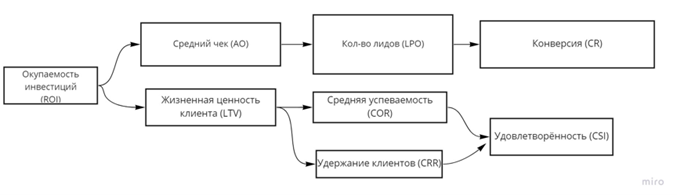
\includegraphics[scale=1.0]{metrics_depandancy.png}
\end{figure}

Здесь продемонстрировано то, по какой логике мы анализируем наш проект. Как было сказано выше, основной показатель -- ROI. По нему мы пониманием состояние нашего проекта. Для более полной детализации мы опускаемся ниже по иерархии показателей: смотрим на средний чек и жизненную ценность клиента и так далее. Также дашборд демонстрирует как показатели влияют друг на друга. 

\subsection{Пример мониторинга показателей по графическим данным (Прототип дашборда)}

Сравним три показателя количество лидов, средний чек и ROI, используя наглядные диаграммы (дашборды). Будет исследована динамика данных показателей за полгода работы сервиса, и показано, как мы выявляем некоторые проблемы нашего сервиса на основе данных метрик.

Здесь продемонстрирована наша основная бизнес-метрика ROI. Мы видим, что показатель рентабельности бизнеса в июне немного упал по сравнению с маем.

\begin{figure}[H]
\centering
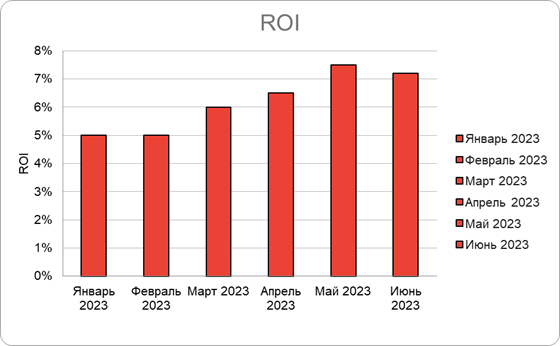
\includegraphics[scale=1.0]{dashboard_roi.png}
\end{figure}

Детализируем данные, спускаясь по иерархии к среднему чеку, чтобы выявить проблему. 

\begin{figure}[H]
\centering
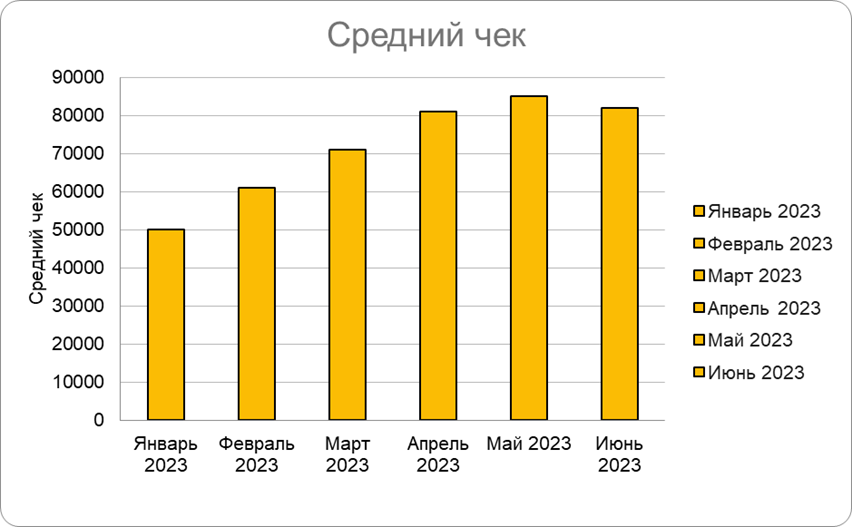
\includegraphics[scale=1.0]{dashboard_check.png}
\end{figure}


Средний чек стабильно рос, в мае было принято решение увеличить цену курсов, и средний чек увеличился до максимума за полгода. Однако в июне он стал снижаться. Спускаемся дальше по иерархии показателей. 

Смотрим на показатель количества людей, совершивших целевое действие.

\begin{figure}[H]
\centering
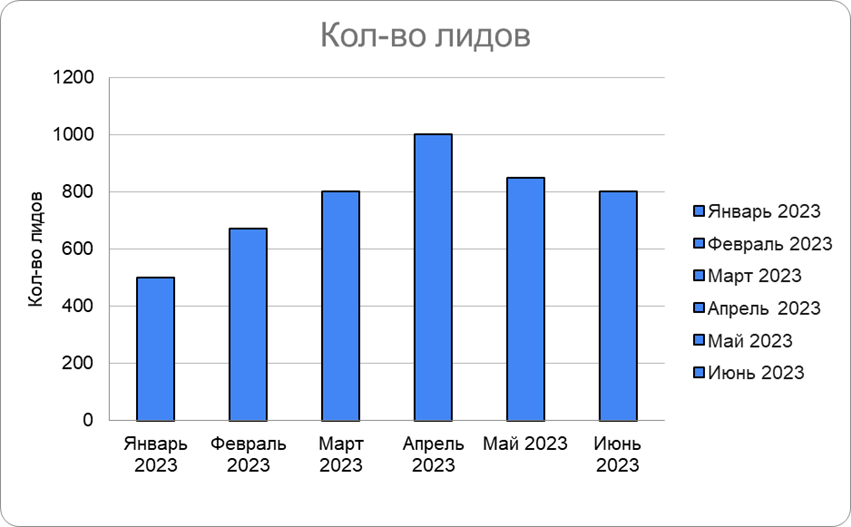
\includegraphics[scale=1.0]{dashboard_action.png}
\end{figure}


Мы видим, что число лидов росло, однако после изменения цены курсов в сторону повышения, их количество уже в следующем месяце сильно сократилось. Значит, наша новая система ценообразования неэффективна, и ее нужно менять в срочном порядке. 

Таким образом, продемонстрирован пример, как мы анализируем состояние нашего проекта и принимаем решения по корректировке конкретных аспектов.

\bibliographystyle{unsrt}
\bibliography{bibl}

\section*{Приложение A. Цифровые материалы}

\subsection{Прототип продукта}

\begin{figure}[H]
\textbf{Прототип главной страницы сервиса}
\centering
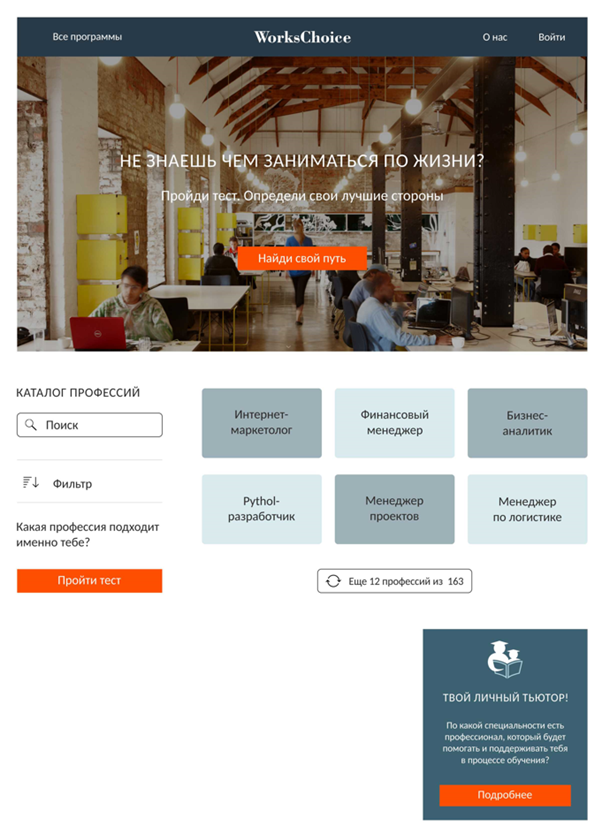
\includegraphics[scale=1.0]{prototype_main.png}
\end{figure}

\begin{figure}[H]
\textbf{Прототип личного кабинета}
\centering
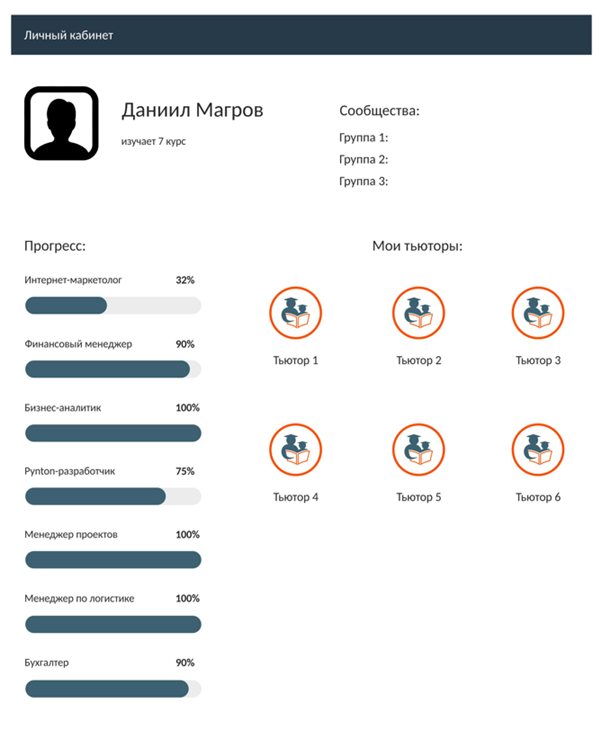
\includegraphics[scale=1.0]{prototype_lk.png}
\end{figure}


\begin{figure}[H]
\textbf{Прототип страницы первой темы профессионального курса}
\centering

\includegraphics[scale=1.0]{prototype_course.png}
\end{figure}

\subsection{Репозиторий}
Используемые иллюстрации, а также .tex файлы для формирования документа можно найти на
\url{https://github.com/chmousNedovolniy/workchoice_project}. 

\end{document}
